\definecolor{tiffanyblue}{RGB}{129,216,208}
\definecolor{bangdiblue}{RGB}{0,149,182}
\definecolor{kleinblue}{RGB}{0,47,167}
\definecolor{kabuliblue}{RGB}{26,85,153}
\definecolor{purple}{RGB}{138,43,226}
\usepgfplotslibrary{groupplots}
\usepgfplotslibrary{fillbetween} 
\begin{figure*}[t!]
  \centering
  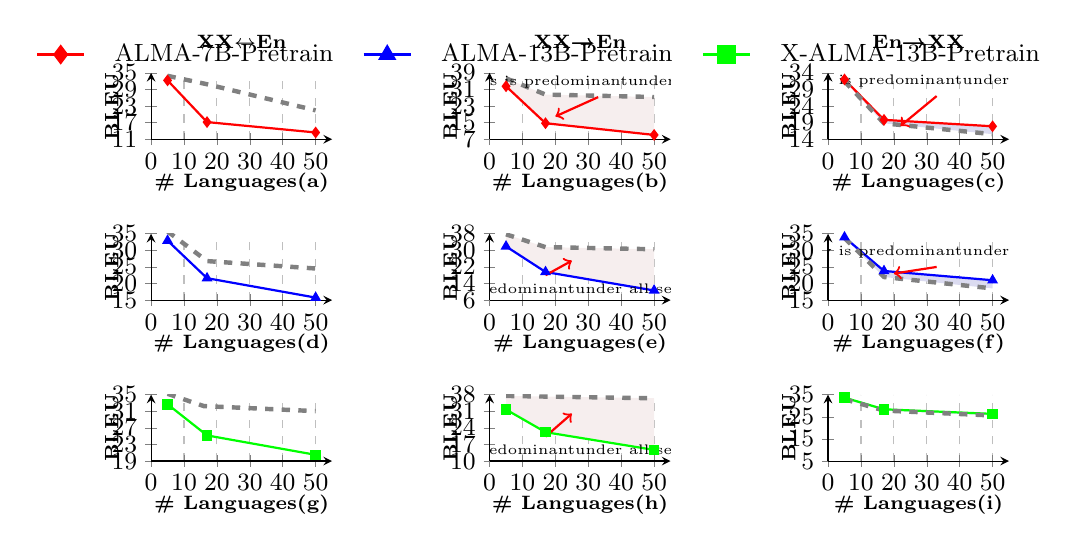
\begin{tikzpicture}
    \pgfplotsset{set layers}
    \scriptsize{
    % 全局图例单独绘制
    \begin{axis}[
    at={(2,1.4)},
    width=0.5\textwidth,
      height=0.2\textwidth,
      hide axis,
      xmin=0, xmax=0.5, ymin=0, ymax=0.5,
      legend style={
        draw=none,
        fill=none,
        font=\small,
        column sep=0.3cm,
        at={(1.1,1.6)},
        anchor=north
      },
      legend columns=3
    ]
      \addlegendimage{red, mark=diamond*, mark size=3.0pt, thick, mark options={solid, fill=red}}
      \addlegendentry{ALMA-7B-Pretrain}
      \addlegendimage{blue, mark=triangle*, mark size=3.0pt, thick, mark options={solid, fill=blue}}
      \addlegendentry{ALMA-13B-Pretrain}
      \addlegendimage{green, mark=square*, mark size=3.0pt, thick, mark options={solid, fill=green}}
      \addlegendentry{X-ALMA-13B-Pretrain}
    \end{axis}
    }
    \scriptsize{
    \begin{groupplot}[
      group style={group size=3 by 3, horizontal sep=2cm, vertical sep=1.2cm},
      xmajorgrids,
      grid style={dashed, gray!50},
      width=0.32\textwidth,
      height=0.2\textwidth,
      xlabel={\# Languages},
      ylabel={BLEU},
      xlabel style={font=\bfseries, yshift=0.5em},
      ylabel style={font=\bfseries, yshift=-1.0em},
      yticklabel style={font=\small},
      xticklabel style={font=\small},
      title style={font=\bfseries},
      xmin=0, xmax=55, 
      xtick={0, 10, 20, 30, 40, 50},
        axis x line=bottom,
        axis y line=left,
        % axis y line*=left, % 左Y轴
    ]
    % 第一行:Model 1
    \nextgroupplot[title={XX$\leftrightarrow$En}, xlabel={\makecell{\# Languages \\ (a) } },ymin=11, ymax=35, ytick={11, 17, 23, 29, 35}]
    \addplot[red, mark=diamond*, mark size=1.5pt, thick, mark options={solid, fill=red}] 
      coordinates {(5, 32.262) (17, 17.199) (50, 13.442)};
    \addplot[ultra thick, dashed, gray] 
      coordinates {(5, 33.9105) (17, 30.875) (50, 21.4365)};
      
    \nextgroupplot[title={XX→En}, xlabel={\makecell{\# Languages \\ (b) } }, ymin=7, ymax=39, ytick={7, 15, 23, 31, 39}]
    \addplot[name path=mt_b,red, mark=diamond*, mark size=1.5pt, thick, mark options={solid, fill=red}] 
      coordinates {(5, 32.525) (17, 14.722) (50, 9.077)};
    \addplot[name path=separate_b,ultra thick, dashed, gray] 
      coordinates {(5, 36.348) (17, 28.524) (50, 27.344)};
    
    \addplot [
        fill=red!30!gray!10
    ] fill between [
        of=mt_b and separate_b,
    ];

    \draw[->, thick, color=red] (axis cs:33,27.3) node[above]{\tiny \textcolor{black}{\makecell{Conflicts is predominant\\ under all settings}}} -- (axis cs:20,18);


    
    \nextgroupplot[
        title={En→XX}, 
        xlabel={\makecell{\# Languages \\ (c) } }, 
        % 左 Y 轴(COMET-22)
        ylabel={BLEU}, 
        ymin=14, ymax=34, 
        ytick={14, 19, 24, 29, 34},
    ]
    \addplot[name path=mt_c, red, mark=diamond*, mark size=1.5pt, thick, mark options={solid, fill=red}] 
      coordinates {(5, 32.0) (17, 19.841) (50, 17.899)};
    \addplot[name path=separate_c,ultra thick, dashed, gray] 
      coordinates {(5, 31.473) (17, 18.793) (50, 15.529)};

    \addplot [
        fill=blue!40!gray!20
    ] fill between [
        of=mt_c and separate_c,
    ];

    \draw[->, thick, color=red] (axis cs:33,27) node[above]{\tiny \textcolor{black}{\makecell{Synergy is predominant\\ under all settings}}} -- (axis cs:22,18)
         ;

   
    
    
    % 第二行:Model 2
    \nextgroupplot[xlabel={\makecell{\# Languages \\ (d) } }, ymin=15, ymax=35, ytick={15, 20, 25, 30, 35}]
    \addplot[blue, mark=triangle*, mark size=1.5pt, thick, mark options={solid, fill=blue}] 
      coordinates {(5, 32.918) (17, 21.611) (50, 15.768)};
    
    % \addplot[ultra thick, dashed, gray] 
    %   coordinates {(5, 88.40) (9, 88.57) (17, 81.692) (50, 78.80)};

    \addplot[ultra thick, dashed, gray] 
      coordinates {(5, 35.715) (17, 26.7595) (50, 24.527)};
    
    \nextgroupplot[xlabel={\makecell{\# Languages \\ (e) } }, ymin=6, ymax=38, ytick={6, 14, 22, 30, 38}]
    \addplot[name path=mt_e, blue, mark=triangle*, mark size=1.5pt, thick, mark options={solid, fill=blue}] 
      coordinates {(5, 31.898) (17, 19.572) (50, 10.649)};

    % \addplot[ultra thick, dashed, gray] 
    %   coordinates {(5, 87.92) (9, 88.068) (17, 84.289) (50, 83.079)};
      \addplot[name path=separate_e, ultra thick, dashed, gray] 
      coordinates {(5, 37.728) (17, 31.551) (50, 30.524)};

     \addplot [
        fill=red!30!gray!10
    ] fill between [
        of=mt_e and separate_e,
    ];

    \draw[->, thick, color=red] (axis cs:17,18) node[below]{\tiny \textcolor{black}{\makecell{Conflicts is predominant\\ under all settings}}} -- (axis cs:25,25)
         ;
     
    \nextgroupplot[xlabel={\makecell{\# Languages \\ (f) } },ymin=15, ymax=35, ytick={15, 20, 25, 30, 35}]
    \addplot[name path=mt_f,blue, mark=triangle*, mark size=1.5pt, thick, mark options={solid, fill=blue}] 
      coordinates {(5, 33.938) (17, 23.787) (50, 20.993)};

     % \addplot[ultra thick, dashed, gray] 
     %  coordinates {(5, 88.882) (9, 89.071) (17, 79.095) (50, 74.52)};

      \addplot[name path=separate_f,ultra thick, dashed, gray] 
      coordinates {(5, 33.702)  (17, 21.968) (50, 18.53)};

      \addplot [
        fill=blue!40!gray!20
    ] fill between [
        of=mt_f and separate_f,
    ];

    \draw[->, thick, color=red] (axis cs:33,25) node[above]{\tiny \textcolor{black}{\makecell{Synergy is predominant\\ under all settings}}} -- (axis cs:20,23)
         ;

    % 第三行:Model 3
    \nextgroupplot[xlabel={\makecell{\# Languages \\ (g) } }, ymin=19, ymax=35, ytick={19, 23, 27, 31, 35}]
    \addplot[green, mark=square*, mark size=1.5pt, thick, mark options={solid, fill=green}] 
      coordinates {(5, 32.685) (17, 25.176) (50, 20.499)};
    \addplot[ultra thick, dashed, gray]  coordinates {(5, 35.1965) (16, 32.242) (50, 31.0265)};

    
    \nextgroupplot[xlabel={\makecell{\# Languages \\ (h) } }, ymin=10, ymax=38, ytick={10, 17, 24, 31, 38}]
    \addplot[name path=mt_h,green, mark=square*, mark size=1.5pt, thick, mark options={solid, fill=green}] 
      coordinates {(5, 31.72) (17, 22.175) (50, 14.693)};
    \addplot[name path=separate_h, ultra thick, dashed, gray] 
      coordinates {(5, 37.445) (50, 36.475)};

      
    % \node at (0.5,-10.25) {(c) XX-En};

    \addplot [
        fill=red!30!gray!10
    ] fill between [
        of=mt_h and separate_h,
    ];

    \draw[->, thick, color=red] (axis cs:17,20.3) node[below]{\tiny \textcolor{black}{\makecell{Conflicts is predominant\\ under all settings}}} -- (axis cs:25,30)
         ;
    
    \nextgroupplot[xlabel={\makecell{\# Languages \\ (i) } },ymin=5, ymax=35, ytick={5, 15,25, 35}]
    \addplot[name path=mt_i,green, mark=square*, mark size=1.5pt, thick, mark options={solid, fill=green}] 
      coordinates {(5, 33.65) (17, 28.377) (50, 26.306)};
      \addplot[name path=separate_i, ultra thick, dashed, gray]  coordinates {(5, 32.948) (17, 27.806)(50, 25.578)};

    \addplot [
        fill=blue!40!gray!20
    ] fill between [
        of=mt_i and separate_i,
    ];

    
    \end{groupplot}
    }
  \end{tikzpicture}
  \vskip -0.1in
  \caption{Performance of different models trained on varying numbers of languages (evaluated by SacreBLEU). The dotted line represents the performance of separately trained models, serving as a reference point where no language conflicts or synergies occur. Two key findings emerge: (1) Asymmetry in Linguistic Conflicts and Synergy (Figure a–i), highlighting the uneven impact of multilingual training across language pairs; and (2) The Bottleneck of Multilinguality in Post-Training (Figure g–i), showing that while monolingual pre-training provides an ideal foundation for handling multiple languages, the post-training stage imposes constraints that lead to the curse of multilinguality.}
  \label{fig:Asymmetric_Conflict_and_Synergy_bleu}
\end{figure*}

